
%%% Local Variables:
%%% mode: latex
%%% TeX-master: t
%%% End:

\chapter{引言}
\label{cha:intro}


\section{选题背景}
\label{sec:background}

21世纪的最初十年是计算机技术与互联网应用发展极为迅速的时期。在此期间,人们见证了CPU主频步入GHz时代,内存的容量和吞吐率按部就班地翻番,硬盘容量进入了TB级,人们探索互联网的接入方式也从曾经的56kbps甚至更慢的modem换成了带宽以Mbps计的宽带接入。可以说,这些都为数字多媒体技术在计算机和互联网上的应用奠定了硬件基础。

我们从十年前看VCD,五年前看DVD,到现在拥有了720p到1080p的高清电影资源;从8bit的音频到24bit、192kHz采样的无损音乐格式,无不需要计算能力更强和存储容量更大的计算机来处理。信息化的大步跨越让多媒体技术在我们日常生活中扮演越来越重要的角色。各种新的应用也接踵而来。

%3D电视的发展
3D电视经过多年的发展,已经逐渐走向成熟。在CES(Consumer Electronics Show) 2010的展厅里,“3D”成了最大的赢家,备受关注。Panasonic的VT25平板3D电视也获得了这届CES的“Best in Show Award”。无论是各大家电厂商展台上的3D电视,还是可以用在现有系统上的nVidia 3D Vision套装,都令消费者们感受到了3D时代即将来临。其实,3D电视的起源并不比2D电视晚很长时间\cite{smolic2007coding},但是由于其对计算、存储和传输的资源消耗比普通2D电视高出一倍甚至数倍,所以一直以来未能普及。

%3D视频编码的发展
为了满足资源有限条件下的3D视频应用,各种编码技术陆续诞生,以一定量的比特率来描述多视频信号,达到一定的压缩率,同时尽可能减小失真。在这个过程中,国际标准化组织应运而生。目前国际上有两个音视频编码标准化组织:
\begin{itemize}
\item 一是国际电信联盟标准化组(ITU-T)下属的视频编码专家组(VCEG:Video Coding Expert Group)。制定了一系列视频通信协议和标准,包括H.261、H.263、H.263+、H.264等。主要应用在视频通信领域,如视频会议等。
\item 二是国际标准化组织(ISO)和国际电工委员会(IEC)下属的运动图像编码专家组(MEPG:Motion Picture Expert Group)。自1988年成立以来,研究和开发了多种多媒体压缩标准,包括MPEG-1、MPEG-2、MPEG-4、MPEG-7等。主要应用在存储媒介(DVD)、广播电视网、有流媒体传输等。
\end{itemize}
\begin{figure}[htbp]
\begin{center}
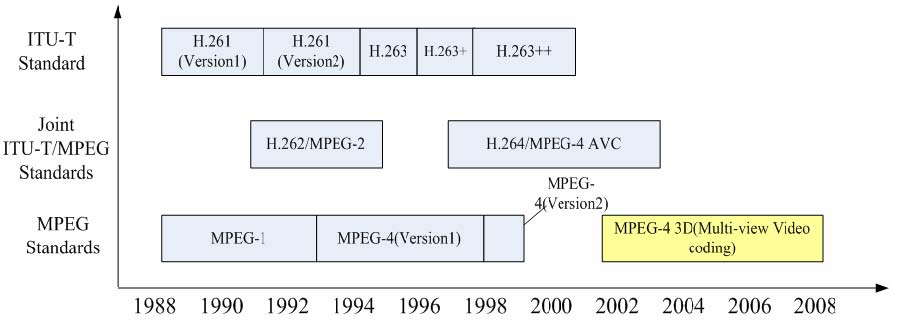
\includegraphics[width=\textwidth]{codecroadmap.png}
\caption{MPEG、VCEG、JVT视频编解码标准的发展}
\label{fig:codecroadmap}
\end{center}
\end{figure}

在2001年6月,经过评估发现,H.26L编码技术基本能够满足MPEG的标准需求,因此MPEG与VCEG的成员共同成立了一个新的工作组JVT(Joint Video Team),来推动和管理H.26L的最后标准化开发,并在2003年形成了视频标准,同时被MPEG和VCEG采纳:MPEG将其定为MEEG-4 part 10,VCEG将其定为H.264。MPEG和VCEG制定的主要标准见。H.264/MPEG-4 part 10标准称为高级视频编码(AVC:Advanced Video Coding),扩展性较好,用于3D视频的多视点视频编解码(MVC:Multi-view Video Coding)就是其一个扩展。MPEG与VCEG及JVT制定的主要视频标准如图\ref{fig:codecroadmap}所示。

\section{已有研究}
\label{sec:previouswork}

%MVC相关工作

在Multi-view Video Coding方向的研究在很久前就开始了。3D视频的一个特点是:传输给用户的各个视角的视频描述的是同一个场景。各个视角的视频在统计意义上的相关性很大,这些相关性就可以用来做预测,如图\ref{fig:mvcpredstruct}所示\footnote{\href{http://mpeg.chiariglione.org/technologies/mpeg-4/mp04-mvc/image004.jpg}{http://mpeg.chiariglione.org/technologies/mpeg-4/mp04-mvc/image004.jpg}}。综合利用时间序列以及视角间的图像预测结构,能够极大地提高编码效率\cite{merkle2005statistical,kaup2006analysis}。\onlinecite{magnor2003multi}中提及了多视点图像编码的一些前沿研究。
\begin{figure}[htbp]
\begin{center}
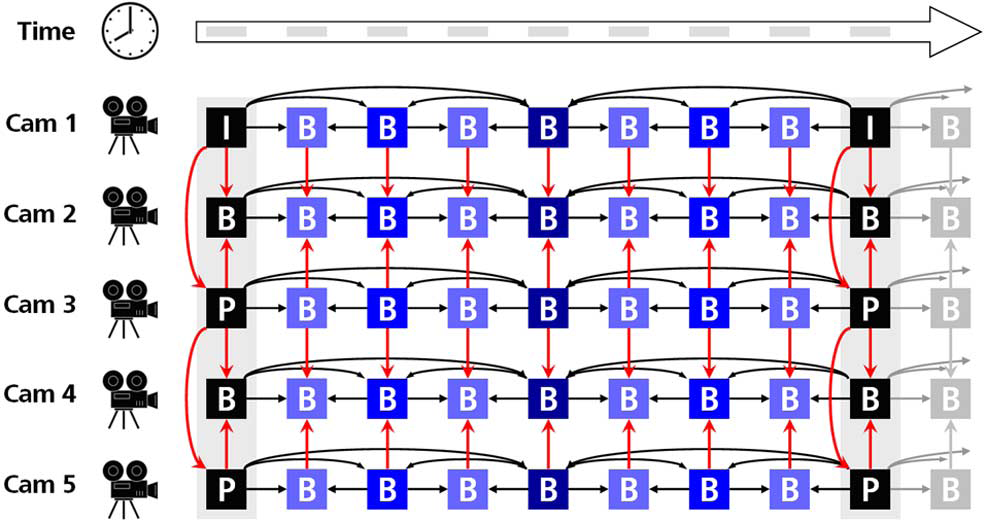
\includegraphics[width=\textwidth]{mvcpredstruct.png}
\caption{MVC的时间和视角间预测结构}
\label{fig:mvcpredstruct}
\end{center}
\end{figure}

对于视角间和时间序列上的图像预测结构,有不少文献提出了不同的方法。其中,H.264/AVC时间和视角间预测的基于B帧的算法\cite{kaup2006analysis}在MPEG标准测试下性能表现最好\cite{flierl2007motion,merkle2006efficient,mueller2006multi,merkle2007efficient}。在实验中,各种指标都显示MVC远远超越了独立压缩每个视角视频的方法。不过,能够获得的性能提升对参数有一定依赖,如相机间距、帧率、内容复杂度(运动和纹理)等属性。对于一些数据集,信噪比峰值(PSNR)的增益在0.5dB以下,而最大的增益能达到3dB。

这个方法在提高视频编码压缩率的同时,增加了编解码的复杂度,要求处理更大量的数据和进行更多的计算。对于MVC编解码的研究大多使用参考软件JMVC进行\footnote{由Heiko Schwarz、Tobias Hinz、Karsten Suehring等人开发。}。参考软件的编写比较注重对应多视点视频编码的原理,对于学习MVC编解码很有帮助,但也因此损失了极大的性能。在实验所使用的机器上对720$\times$576的两路视频进行编码,19帧需要大约半个小时,这远远不够实际应用的需求。诺基亚研究中心(Nokia Research Center)针对其运行Maemo的平台开发了一款MVC实时解码器\footnote{\href{http://research.nokia.com/research/mobile3D}{http://research.nokia.com/research/mobile3D}},针对单核心做了不少优化。由于其主要利用汇编优化,而处理器并不是x86兼容的,所以不易移植到PC上。

至此,我们认为有必要进行一个能够在PC上进行两路到更多路MVC视频的解码器,进行客户端的实时解码。这样的解码器是3D视频应用普及的一个重要前提。

由于MVC是H.264/AVC的一个扩展,所以我们首先想到H.264的并行编解码问题。这个方向近几年有一些文献:\onlinecite{li2005design}提出的算法使用一个处理器进行动量估计以外的运算,其余处理器进行运动向量的估计。\onlinecite{seitner2007macroblock}做了H.264解码器的宏块并行分析,\onlinecite{mesa2009scalability}给出了H.264解码器宏块并行算法。而更进一步针对多视点视频的并行解码的研究相对较少:\onlinecite{yang2006parallel}提出了一种超空间(hyper-space)的方法,\onlinecite{ugur2007parallel}通过对参考帧施加一定限制条件使得解码器等待参考帧传入的时间大幅降低,从而提升并行解码速度。

%庞一等 论文
庞一等在2009年提出了一种多核架构上并行处理多视点视频的启发式调度框架\cite{pang2009framework}。不同于以往的帧并行或宏块并行的研究,提出了通过优化解码任务调度来提高解码器并行性能的观点,并通过实验证明性能的大幅提升。该方法对多视点视频的调度如图\ref{fig:gopschedulinginmvc}所示,通过重新安排帧解码顺序,最小化多路视频解码时因为等待参考帧传入和其解码结果的等待时间,从而加快解码速度。
\begin{figure}[htbp]
\begin{center}
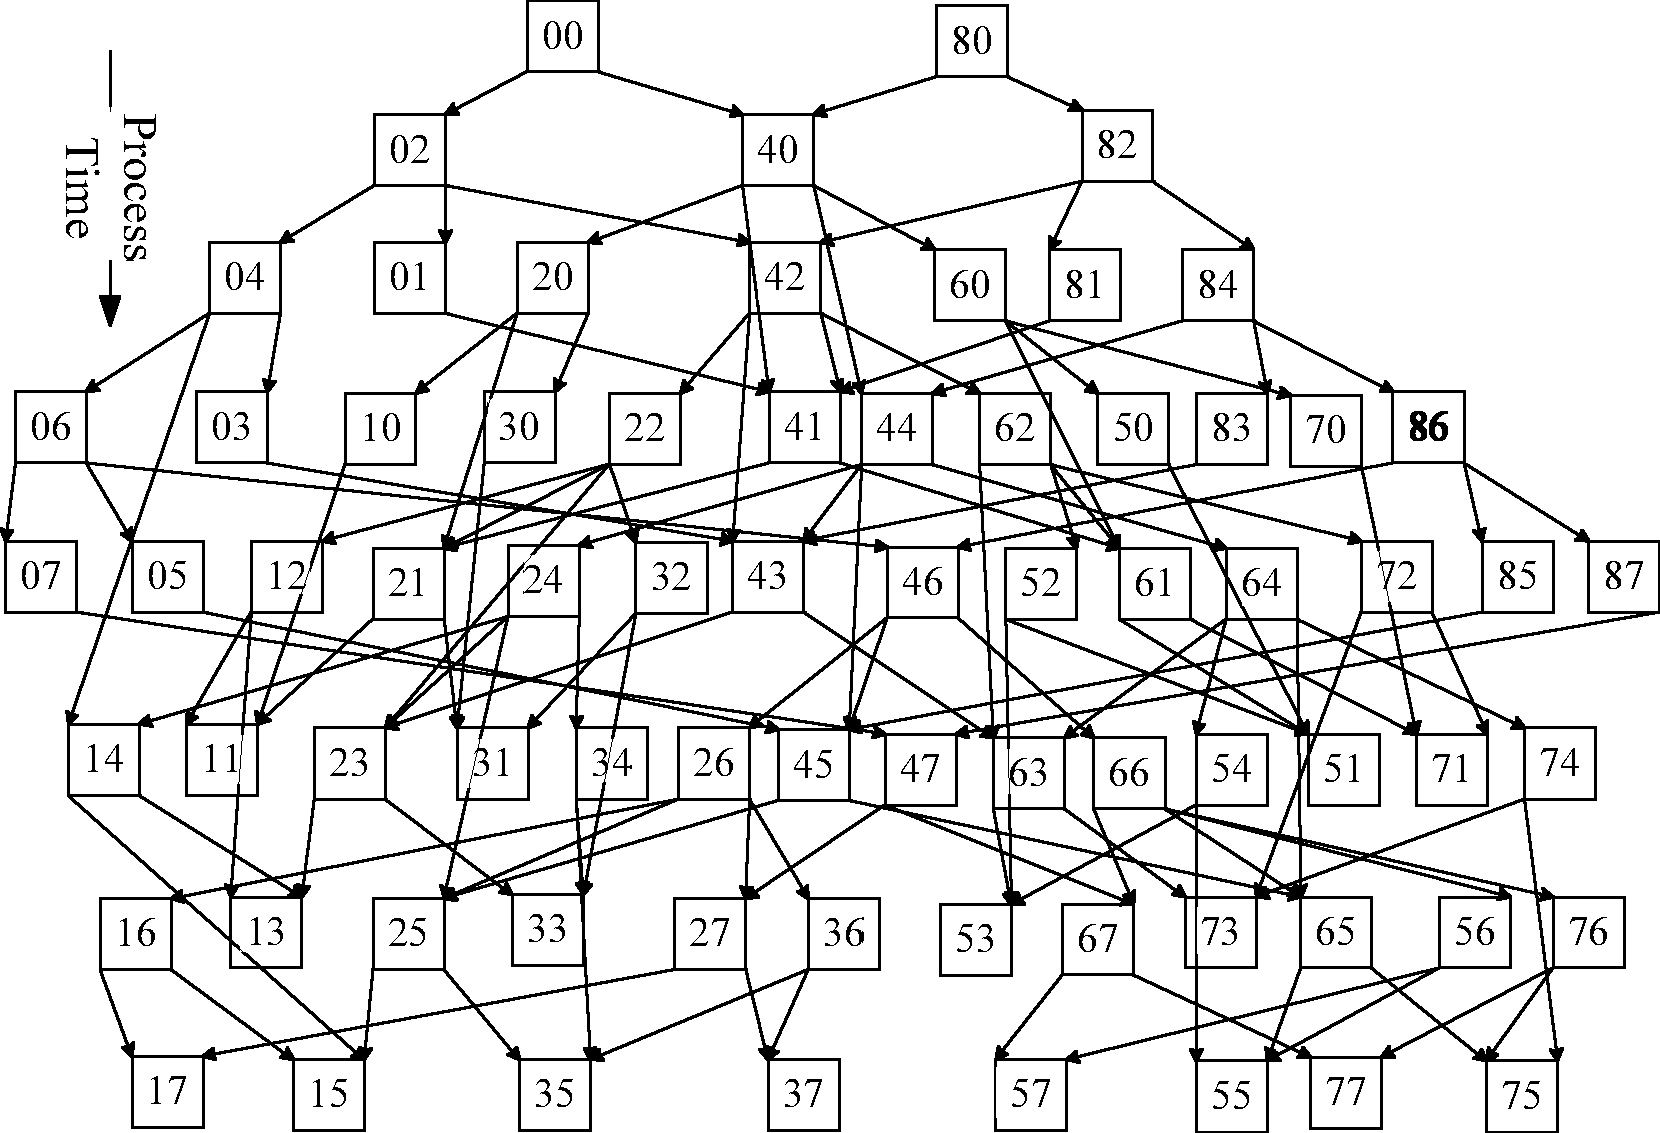
\includegraphics[width=\textwidth]{gopschedulinginmvc.png}
\caption{多视点视频种的GOP调度}
\label{fig:gopschedulinginmvc}
\end{center}
\end{figure}


%MVC Decoder工作
在此基础上,我们已经实现了一个成型的多视点视频编解码系统,包括编码器和解码器。编码器将若干YUV格式的视频编码为一个MVC视频。解码器将一个MVC视频解码为N个独立的YUV视频,N为该MVC视频包含的视角数量。编解码结果符合MVC的标准\cite{iso2009mvc}。

在第\ref{cha:decoderprincipleandrealization}章中将进一步介绍解码器部分。

\section{本文的任务}
\label{sec:workbrief}

目前已有的MVC Decoder工程速度较慢,不能满足实时解码播放的要求。本文主要通过针对单核和多核结构的优化,是现有的MVC解码器能够在CPU上做到至少两路分辨率为720$\times$576的视频的实时解码。

此外,由于MVC视频的标准\cite{iso2009mvc}发布尚不足一年,硬件也尚未普及,还没有一种播放器能够支持各种硬件平台上的MVC视频播放。我们的实验环境有Bolod的3D平板电视和nVidia的3D Vision眼镜套装,为了实现一个从采集到播放的完整系统,除了解码器的优化以外,我还需要设计实现一个3D播放器,让用户能够看到三维的播放效果。

\section{本文的结构}
\label{sec:thesisstructure}

本文第\ref{cha:decoderprincipleandrealization}章介绍需要优化的多视点视频解码器的原理和实现。第\ref{cha:optapproach}章说明我进行解码器性能优化的基本思路。第\ref{cha:singlecoreopt}章和第\ref{cha:parallelopt}章分别详述单核心性能优化和多核处理的并行优化过程。第\ref{cha:optresultandanalysis}章介绍实验结果并进行了一定的分析。同时进行的3D播放器设计与实现部分与解码器优化是两个独立的工作,所以单列在第\ref{cha:3Dplayerdesignandrealization}章。最后在第\ref{cha:conclusionandforesight}章总结解码器优化和3D播放器的工作,并对下一步的工作有所展望。
